\chapter{Movement}

Ships and missiles move only during the movement step of an impulse. Ships move forward relative to their facing; they never move backward.

\section{Ship movement choices}

When a ship's speed appears on the impulse card, choose one legal action:

\begin{itemize}
  \item move forward one hex without changing facing;
  \item side-slip one forward-diagonal hex without changing facing;
  \item turn 60 degrees in place after satisfying turn mode; or
  \item lose the movement if no legal maneuver exists.
\end{itemize}

\begin{center}
\begin{tikzpicture}[
  scale=.78,
  >=Latex
]
  % Flat-top hexes meet across their edges. Their neighboring centers lie at
  % 30, 90, 150, 210, 270, and 330 degrees---not at the vertices.
  \coordinate (forward) at (0,1.022in);
  \coordinate (port) at (-.885in,.511in);
  \coordinate (starboard) at (.885in,.511in);
  \coordinate (west) at (-.885in,-.511in);
  \coordinate (aft) at (0,-1.022in);
  \coordinate (east) at (.885in,-.511in);

  % Draw exact .59-inch-radius hexes so neighboring cells share an edge
  % without the hidden padding introduced by TikZ polygon nodes.
  \foreach \cell in {west,aft,east} {
    \begin{scope}[shift={(\cell)}]
      \draw[reachline]
        (.59in,0) -- (.295in,.511in) -- (-.295in,.511in) --
        (-.59in,0) -- (-.295in,-.511in) -- (.295in,-.511in) -- cycle;
    \end{scope}
  }
  \begin{scope}[shift={(forward)}]
    \draw[reachgold,fill=reachgold!10]
      (.59in,0) -- (.295in,.511in) -- (-.295in,.511in) --
      (-.59in,0) -- (-.295in,-.511in) -- (.295in,-.511in) -- cycle;
  \end{scope}
  \foreach \cell in {port,starboard} {
    \begin{scope}[shift={(\cell)}]
      \draw[reachblue,fill=reachblue!8]
        (.59in,0) -- (.295in,.511in) -- (-.295in,.511in) --
        (-.59in,0) -- (-.295in,-.511in) -- (.295in,-.511in) -- cycle;
    \end{scope}
  }
  \draw[reachgold,line width=1.2pt,fill=reachgold!5]
    (.59in,0) -- (.295in,.511in) -- (-.295in,.511in) --
    (-.59in,0) -- (-.295in,-.511in) -- (.295in,-.511in) -- cycle;

  \draw[->,line width=2pt,reachgold] (0,.18in) -- ($(forward)+(0,-.18in)$);
  \draw[->,densely dashed,line width=1.6pt,reachblue] (-.13in,.08in) -- ($(port)+(.16in,-.09in)$);
  \draw[->,densely dashed,line width=1.6pt,reachblue] (.13in,.08in) -- ($(starboard)+(-.16in,-.09in)$);

  \node[font=\sffamily\small\bfseries,text=reachgold,align=center] at ($(forward)+(0,.18in)$) {FORWARD};
  \node[font=\sffamily\scriptsize\bfseries,text=reachblue,align=center,text width=.82in]
    at ($(port)+(0,.19in)$) {PORT\\SLIP};
  \node[font=\sffamily\scriptsize\bfseries,text=reachblue,align=center,text width=.82in]
    at ($(starboard)+(0,.19in)$) {STARBOARD\\SLIP};

  % The side-slip destinations retain the ship's original north-facing heading.
  % The forward movement arrow already communicates that heading on its own.
  \foreach \cell in {port,starboard} {
    \draw[->,line width=.9pt,reachsteel]
      ($(\cell)+(0,-.34in)$) -- ($(\cell)+(0,-.17in)$);
  }

  \node[inner sep=0pt] at (0,.03in) {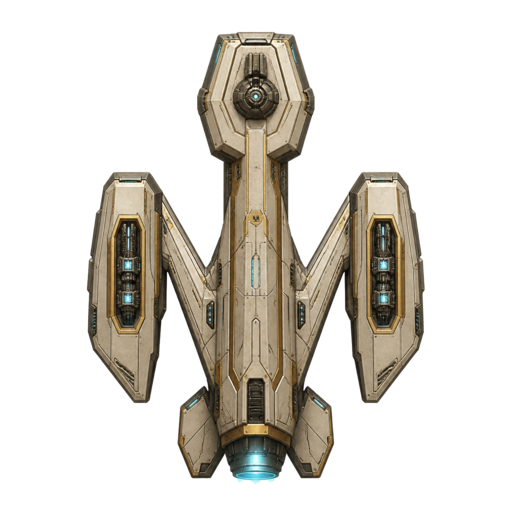
\includegraphics[width=.64in]{../../app/assets/images/ships/tactical/aurelian_frigate.png}};
  \draw[->,line width=1.3pt,reachcopper]
    ($(0,.08in)+(90:.35in)$) arc[start angle=90,end angle=150,radius=.35in];
  \draw[->,line width=1.3pt,reachcopper]
    ($(0,.08in)+(90:.35in)$) arc[start angle=90,end angle=30,radius=.35in];
  \node[font=\sffamily\scriptsize\bfseries,text=reachcopper,align=center]
    at (0,-.42in) {TURN 60\textdegree};
  \node[font=\sffamily\scriptsize,text=reachblue,align=center] at (0,-1.78in)
    {DASHED ARROW: move to another hex; keep facing north};
  \node[font=\sffamily\scriptsize,text=reachcopper,align=center] at (0,-1.98in)
    {CURVED ARROW: remain in the hex; rotate 60\textdegree};
\end{tikzpicture}
\end{center}

\section{Turn mode}

A ship's \term{turn mode} is the number of hexes it must translate forward before it may turn again. Moving forward and side-slipping both add one to this count. Turning resets the count to zero.

\begin{center}
\begin{tabular}{lccc}\toprule
Hull class & Speed 1--4 & Speed 5--8 & Speed 9--12\\\midrule
Small & 0 & 1 & 2\\
Medium & 1 & 2 & 3\\
Large & 2 & 3 & 4\\\bottomrule
\end{tabular}
\end{center}

A speed-0 ship does not receive a normal movement opportunity. A turn mode of 0 permits a ship to turn on every movement opportunity, including repeatedly turning in place under the standard rules.

\section{Side-slipping}

A side-slip moves the ship into either forward-diagonal hex while preserving its facing. It represents a more granular course change than the hex grid otherwise permits.

A ship may not side-slip twice in succession. It must move forward or turn before it may side-slip again. A side-slip counts as forward movement for satisfying turn mode.

\section{Occupied hexes and the map edge}

A ship may never enter a hex occupied by another ship. It must choose another legal movement or turn if possible, using its special maneuver if necessary and available. If no legal choice exists, the movement is lost.

Missiles may share hexes with ships and other missiles. A missile that enters its assigned target's hex immediately impacts.

A ship that leaves the map for any reason is destroyed for all purposes, including victory scoring.

\section{Missile movement}

Missiles move at speed 24: two one-hex moves during the movement step of every impulse. They have turn mode 0 and must use each move to approach their assigned target. If a missile reaches the target after its first hex of movement, it impacts immediately and does not take a second move.

Missiles launch \emph{after} movement. A newly launched missile is placed in its launching ship's hex and does not move during that impulse. It begins moving in the following impulse. If its target is destroyed before impact, the missile loses lock and is removed.

\section{Special maneuvers}

Every small and medium ship begins the game with one special-maneuver token. Large ships do not. The token may be spent once per game during that ship's movement opportunity, either immediately before or immediately after its normal movement.

\begin{description}[style=nextline,leftmargin=0pt]
  \item[Bootlegger] Rotate the ship to any facing, ignoring normal turn-mode restrictions. This counts as a turn and resets forward hexes accumulated toward the next turn.
  \item[Quick Stop] Set the ship's speed to 0. It receives no more normal movement opportunities that turn.
  \item[Emergency Power] Immediately move one extra hex straight forward. The destination must be open.
\end{description}

Once spent, the token is unavailable for the rest of the battle.
